%-------------------------------------------------------------------------------
% Autores: I. R. Pagnossin e Centro de Ensino e Pesquisa Aplicada.
%
% Este material é parte integrante do curso "Usando LaTeX; pensando em TeX" e é
% distribuido pelos autores segundo a licença Creative Commons 2.5 Brasil
% (atribuição/não-comercial/redistribuição segundo a mesma licença).
%
% This material is part of the course "Usando LaTeX; pensando em TeX".
% It is distributed according to the license Creative Commons 2.5 Brazil
% (attribution/non-comercial use/share alike the same license).
%-------------------------------------------------------------------------------
\newif\ifhandout
%\handouttrue  % Descomente se for para gerar a versão para IMPRESSÃO.
\handoutfalse % Descomente se for para gerar a versão para APRESENTAÇÃO

%-------------------------------------------------------------------------------
\ifhandout
  \documentclass[handout,10pt]{beamer}
  \mode<handout>
\else
	\documentclass[10pt,hyperref={pdfpagelabels=false}]{beamer}
	\mode<presentation>
\fi

	\usepackage[ansinew]{inputenc}
	\usepackage{ae}
	\usepackage{bookman}
	\usepackage{helvet}	
	\usepackage{lipsum}
	\usepackage{tabularx}
	\usepackage{calc}
	\usepackage{multirow}
	\usepackage[brazil]{babel}	
	\usepackage{graphicx}
	\usepackage{listings}
	\usepackage{tikz}
	\usepackage{amsmath}
	\usepackage[squaren]{SIunits}
	\usepackage{booktabs}
	\usepackage{fancybox}
	\usepackage{array}
	\usepackage{colortbl}
	
	\ifhandout
		\usepackage{pgfpages}
		\pgfpagesuselayout{2 on 1}[a4paper,border shrink=5mm]
	\fi

	% Bibliotecas TikZ e PGF necessárias
	\usetikzlibrary{shapes.symbols}
	\usetikzlibrary{calc}
	\usepgflibrary{shapes.misc}
	
	% Configurações pessoais
	% Configurações personalizadas do código LaTeX.	
\lstnewenvironment{LaTeXcode}{
	\setlength{\abovecaptionskip}{0pt}	
	\lstset{language=[LaTeX]TeX}
	\lstset{%
		basicstyle=\footnotesize\ttfamily,  % Global
		keywordstyle=\color{blue}\bfseries, % Comandos
		identifierstyle=,                   % Texto
		stringstyle=,                       % Strings 
		commentstyle=\color{gray},          % Comentários
		showstringspaces=false,             % Espaços
		rulecolor=\color{gray},             % Linha da caixa
	}
	\lstset{emph={setlength,includegraphics,psfrag,subfigure},emphstyle={\color{blue}\bfseries}}
}% Abrindo o ambiente.
{}% Fechando o ambiente.
	
\newcommand{\digite}[1]{{\fontfamily{cmss}\fontseries{bx}\selectfont#1}}	
\newcommand{\cs}[1]{{\normalfont\textbackslash\color{blue!50!black}#1}}
\newcommand{\pkg}[1]{{\normalfont\sffamily\color{orange}#1}}
\newcommand{\env}[1]{{\normalfont\sffamily\color{green!50!black}#1}}
\let\comando=\cs
\let\package=\pkg
\let\ambiente=\env
\newcommand{\foreign}[1]{{\textsl{#1}}}


	\newcounter{exercicio}	
	\newenvironment{exercicio}{%
		\refstepcounter{exercicio}%
		\penalty-200
		\noindent\colorbox{blue!60!black}{\makebox[\columnwidth-\fboxsep*2][c]{\textbf{\color{white}Exercício~\theexercicio}}}\smallskip
	}{\par\medskip}
		

\newcommand{\bibtex}{\textsc{Bib}\TeX}

\newenvironment<>{atividade}[1]{%
\begin{actionenv}#2%
\begin{exampleblock}{{Atividade #1}}%
}
{%
\end{exampleblock}%
\end{actionenv}%
}


	% Path das figuras, relativo a esta pasta.
	\graphicspath{{../arquivos_comuns/figuras/}{./figuras/}}

	% Modelo da apresentação	
	\usetheme{Frankfurt}
	\usefonttheme{serif,structurebold}
	\setbeamercovered{transparent}		
		
	% Metadados do arquivo PDF.
	\hypersetup{
		pdftitle={BibTeX},
		pdfauthor={Dr. Ivan R. Pagnossin},
		pdfsubject={LaTeX},
		pdfkeywords={TeX,LaTeX}
	}

	% Título, autores e instituição.
	\title{\bibtex}
	\subtitle{e detalhes tipográficos do \LaTeX}
	\author{\textbf{Prof.:} Ivan R. Pagnossin \and \textbf{Tutora:} Juliana Giordano}
	\institute{%
		Coordenadoria de Tecnologia da Informação\\
		Centro de Ensino e Pesquisa Aplicada}
	\logo{
\includegraphics[width=0.25\textwidth]{LogotipoCursoLaTeX_v3_pequeno}}
	\date{}
	
\begin{document}


%-------------------------------------------------------------------
\begin{frame}[c,label=titulo]
	\centering	
	
	
\includegraphics[width=0.8\textwidth]{LogotipoCursoLaTeX_v2}

	\titlepage
\end{frame}
%-------------------------------------------------------------------
\logo{} % <-- O logotipo não aparecerá mais a partir daqui.
\setbeamertemplate{background canvas}{%
		
\includegraphics[width=\paperwidth,height=\paperheight,keepaspectratio=false]{leao-pensador-wattermark.png}
}
%-------------------------------------------------------------------
\newcommand{\cmr}{\usefont{T1}{cmr}{n}{u}}

%-------------------------------------------------------------------
%-------------------------------------------------------------------
\section{\bibtex}
\subsection{A lista thebibliography}

\begin{frame}[fragile]\small	
	\frametitle{Bibliografia ``à mão livre''}	
	\framesubtitle{A lista thebibliography}
		
	\begin{block}{}
		\centering
		\ambiente{thebibliography} é uma lista cujos itens podem ser referenciados
	\end{block}\vfill
	
	\begin{atividade}<2->{1}
	
		\begin{LaTeXcode}
			\begin{thebibliography}{-}
			
			  \bibitem{Kopka:1999}          % Rótulo
			    H. Kopka e P. W. Daly,      % Autor
			    \textsl{A guide to \LaTeX}, % Título
			    Addison-Wesley (1999).      % Editora e data
			  
			  \bibitem{Gratzer:1996}
			    G. Grätzer, \textbf{Math into \LaTeX},
			    \textit{Birkhüaser} (1996).
			  
			\end{thebibliography}
		\end{LaTeXcode}
	\end{atividade}			
\end{frame}
%-------------------------------------------------------------------
\subsection{O comando {\ttfamily\textbackslash cite}}
	
\begin{frame}[fragile]
	\frametitle{Bibliografia ``à mão livre''}	
	\framesubtitle{O comando {\ttfamily\textbackslash cite}}	
	
	\begin{block}{}
		\centering
		\cs{cite}\verb|[|\textit{obs.}\verb|]{|\textit{rótulo(s)}\verb|}|		
	\end{block}
	
	\begin{flushright}
		\footnotesize
		\cs{bibitem} é análogo a \cs{label} e \cs{cite}, a \cs{ref}.
	\end{flushright}\vfill	
	
	\begin{tabbing}
		\hspace{0.6\textwidth}\=\kill
		\cs{cite}\verb|{Kopka:1999}|\>\cite{Kopka:1999}\\
		\cs{cite}\verb|[pp.~15--20]{Kopka:1999}|\>\cite[pp.~15--20]{Kopka:1999}\\
		\cs{cite}\verb|{Kopka:1999,Gratzer:1996}|\>\cite{Kopka:1999,Gratzer:1996}
	\end{tabbing}\vfill
			
	\footnotesize
	\textbf{obs.:} estude o pacote \pkg{natbib}, que expande o comando 
	\cs{cite} e define outros similares. Clique
	\href{http://merkel.zoneo.net/Latex/natbib.php}{aqui} para ver exemplos de
	uso.

\end{frame}
%-------------------------------------------------------------------
\subsection{\bibtex: a idéia}
\begin{frame}
	\frametitle{\bibtex}
	\framesubtitle{A idéia: separar dados bibliográficos do leiaute}
		
	\begin{block}{\ambiente{thebibliography}: leiaute e conteúdo (dados) estão
		\emph{juntos}}
		\centering
		
		\begin{tikzpicture}
			\node [inner sep=5pt,label=150:Conteúdo] {\begin{tikzpicture}
				\fill [red,opacity=0.5] (0,0) circle (1);
			\end{tikzpicture}};
			\node [inner sep=5pt,label=30:Leiaute] at (0.5,0) {\begin{tikzpicture}
				\fill [yellow,opacity=0.5] (0,0) circle (1);
			\end{tikzpicture}};
		\end{tikzpicture}
	\end{block}		
	
	\begin{block}<2->{\bibtex: leiaute e conteúdo (dados) estão \emph{separados}}
		\centering
	
		\begin{tikzpicture}
			\node [name=data,inner sep=5pt,label=150:Conteúdo] {\begin{tikzpicture}
				\fill [red,opacity=0.5] (0,0) circle (1);
			\end{tikzpicture}};
			\node [name=layout,inner sep=5pt,label=30:Leiaute] at (2.5,0)
				{\begin{tikzpicture} \fill [yellow,opacity=0.5] (0,0) circle (1);			
			\end{tikzpicture}};
			
			\node at (layout.center) {\texttt{.bst}};
			\node at (data.center) {\texttt{.bib}};
		\end{tikzpicture}
	\end{block}	
\end{frame}
%-------------------------------------------------------------------
\subsection{Funcionamento}
\begin{frame}
	\frametitle{\bibtex}
	\framesubtitle{Funcionamento}

	\centering

	\includegraphics<1->[height=0.75\textheight]{bibstep1}%
	\llap{\includegraphics<2->[height=0.75\textheight]{bibstep2}}%
	\llap{\includegraphics<3->[height=0.75\textheight]{bibstep3}}	
	
	\vfill
	
	\begin{uncoverenv}<4->
		\begin{center}
			\bibtex\ não é \LaTeX!
		\end{center}
	\end{uncoverenv}
\end{frame}
%-------------------------------------------------------------------
{
\newsavebox{\bibbox}
\savebox{\bibbox}{\raisebox{-0.5\height}[0.5\height][0.25\height]{%
	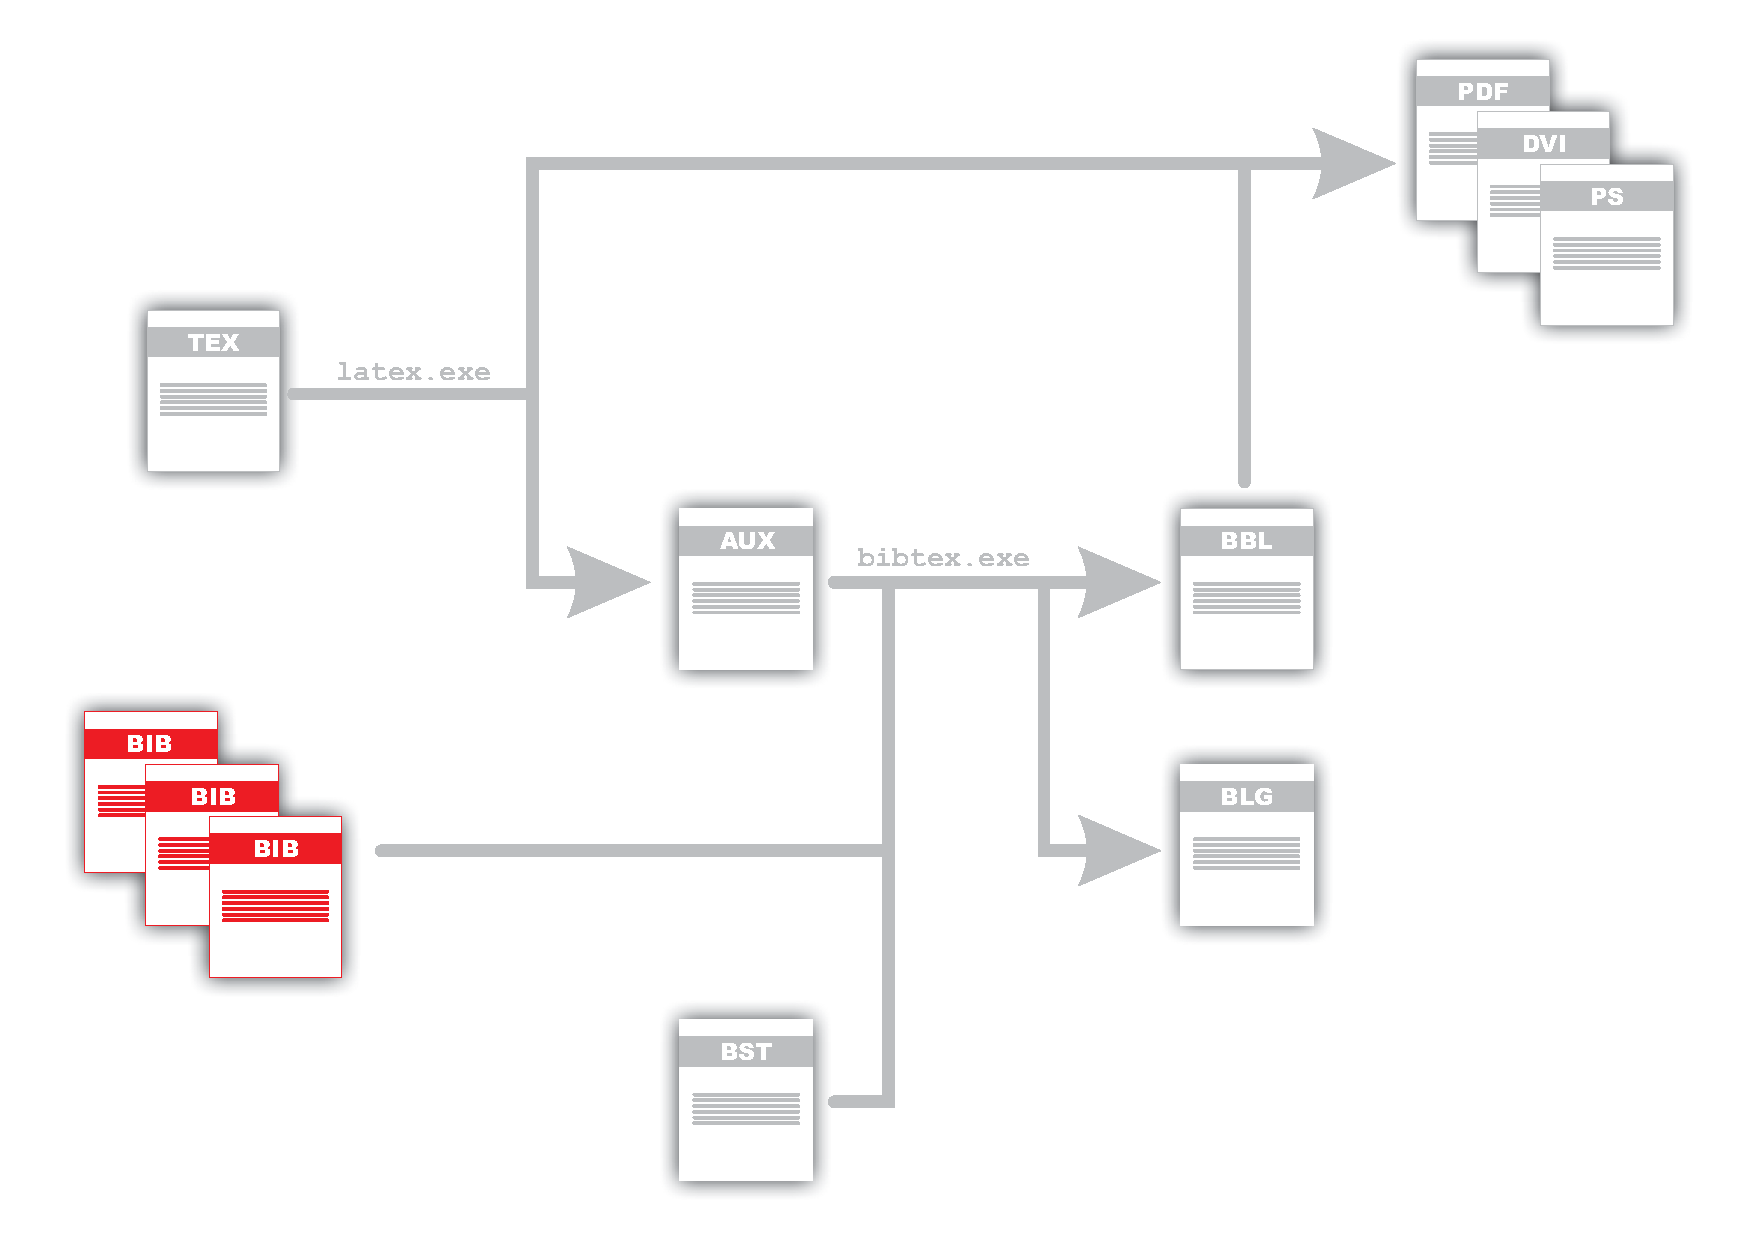
\includegraphics[height=0.55\textheight]{bibfiles_bib}}}
\newsavebox{\bstbox}
\savebox{\bstbox}{\raisebox{-0.5\height}[0.5\height][0.25\height]{%
	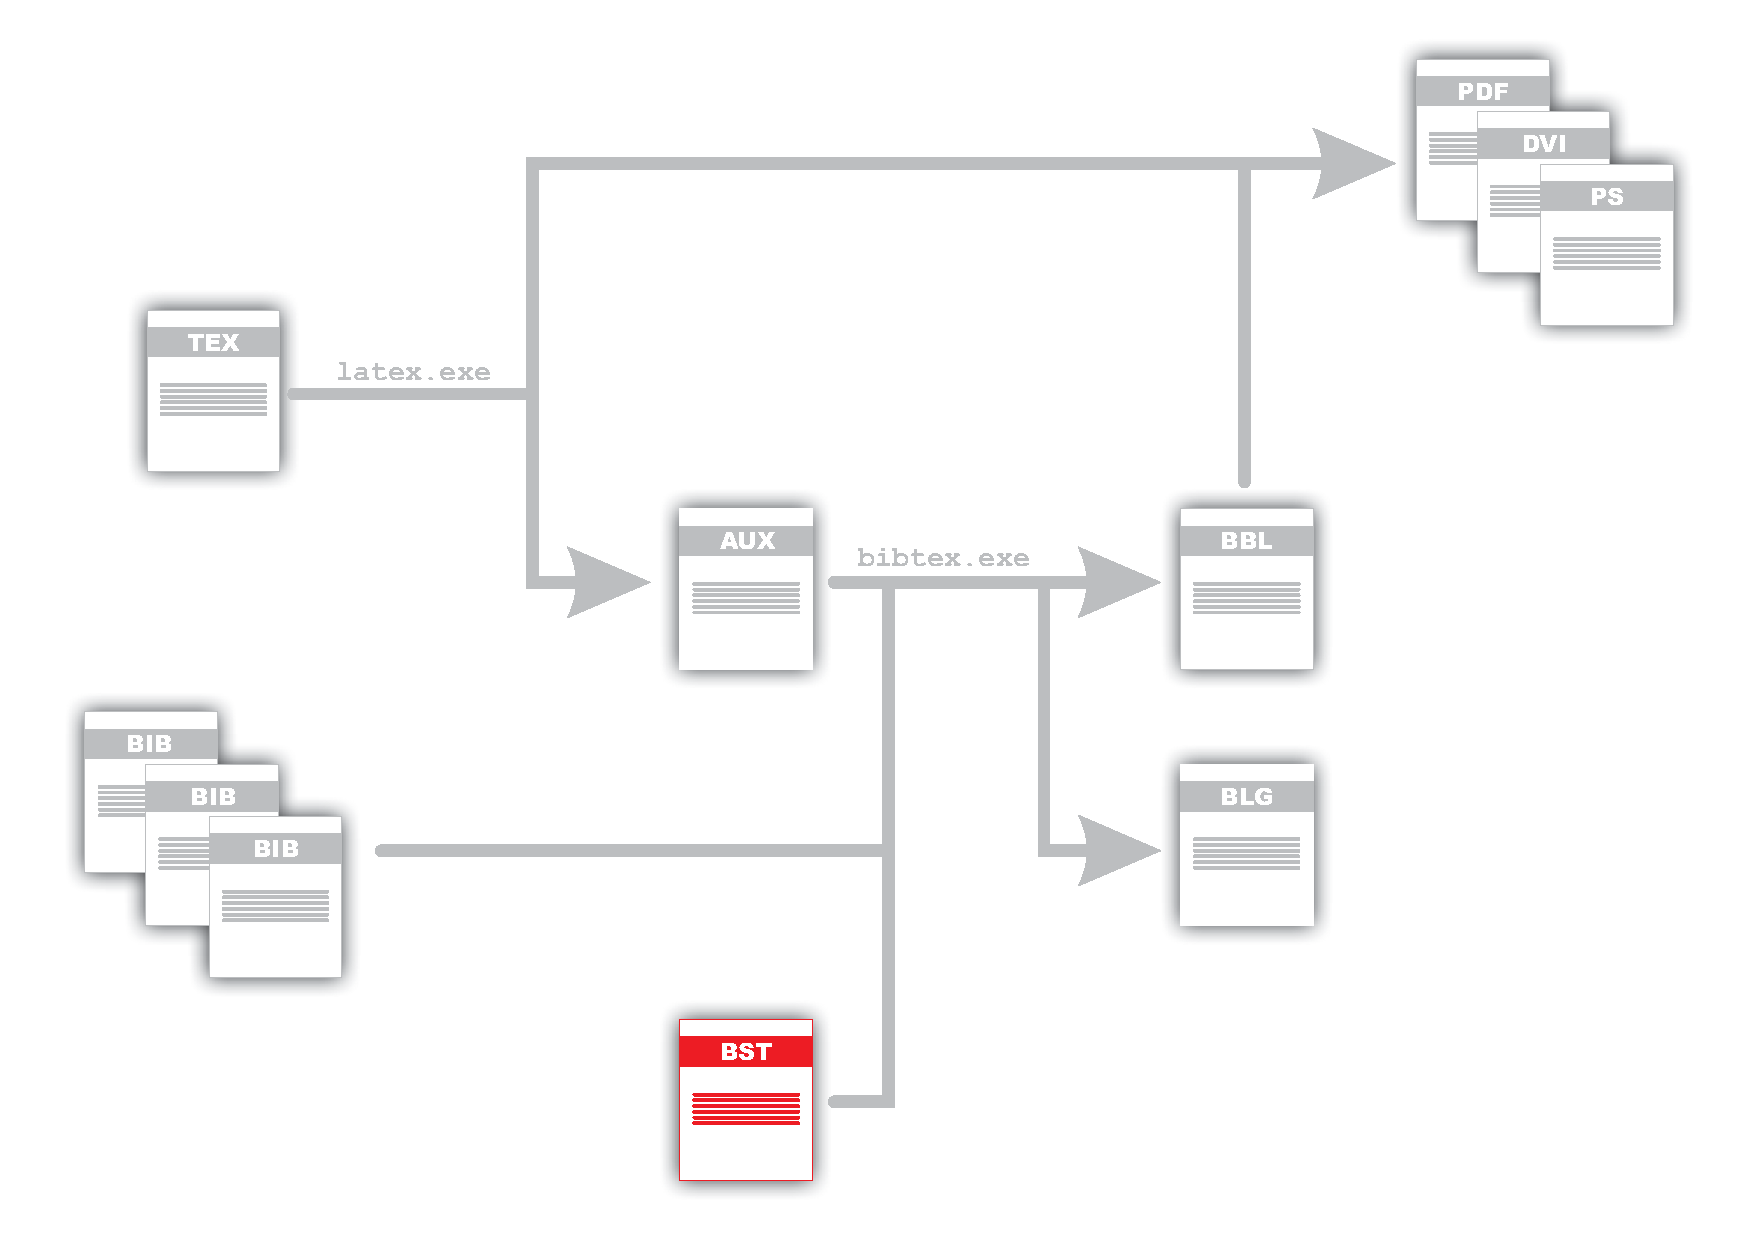
\includegraphics[height=0.55\textheight]{bibfiles_bst}}}
\newsavebox{\bblbox}
\savebox{\bblbox}{\raisebox{-0.5\height}[0.5\height][0.25\height]{%
	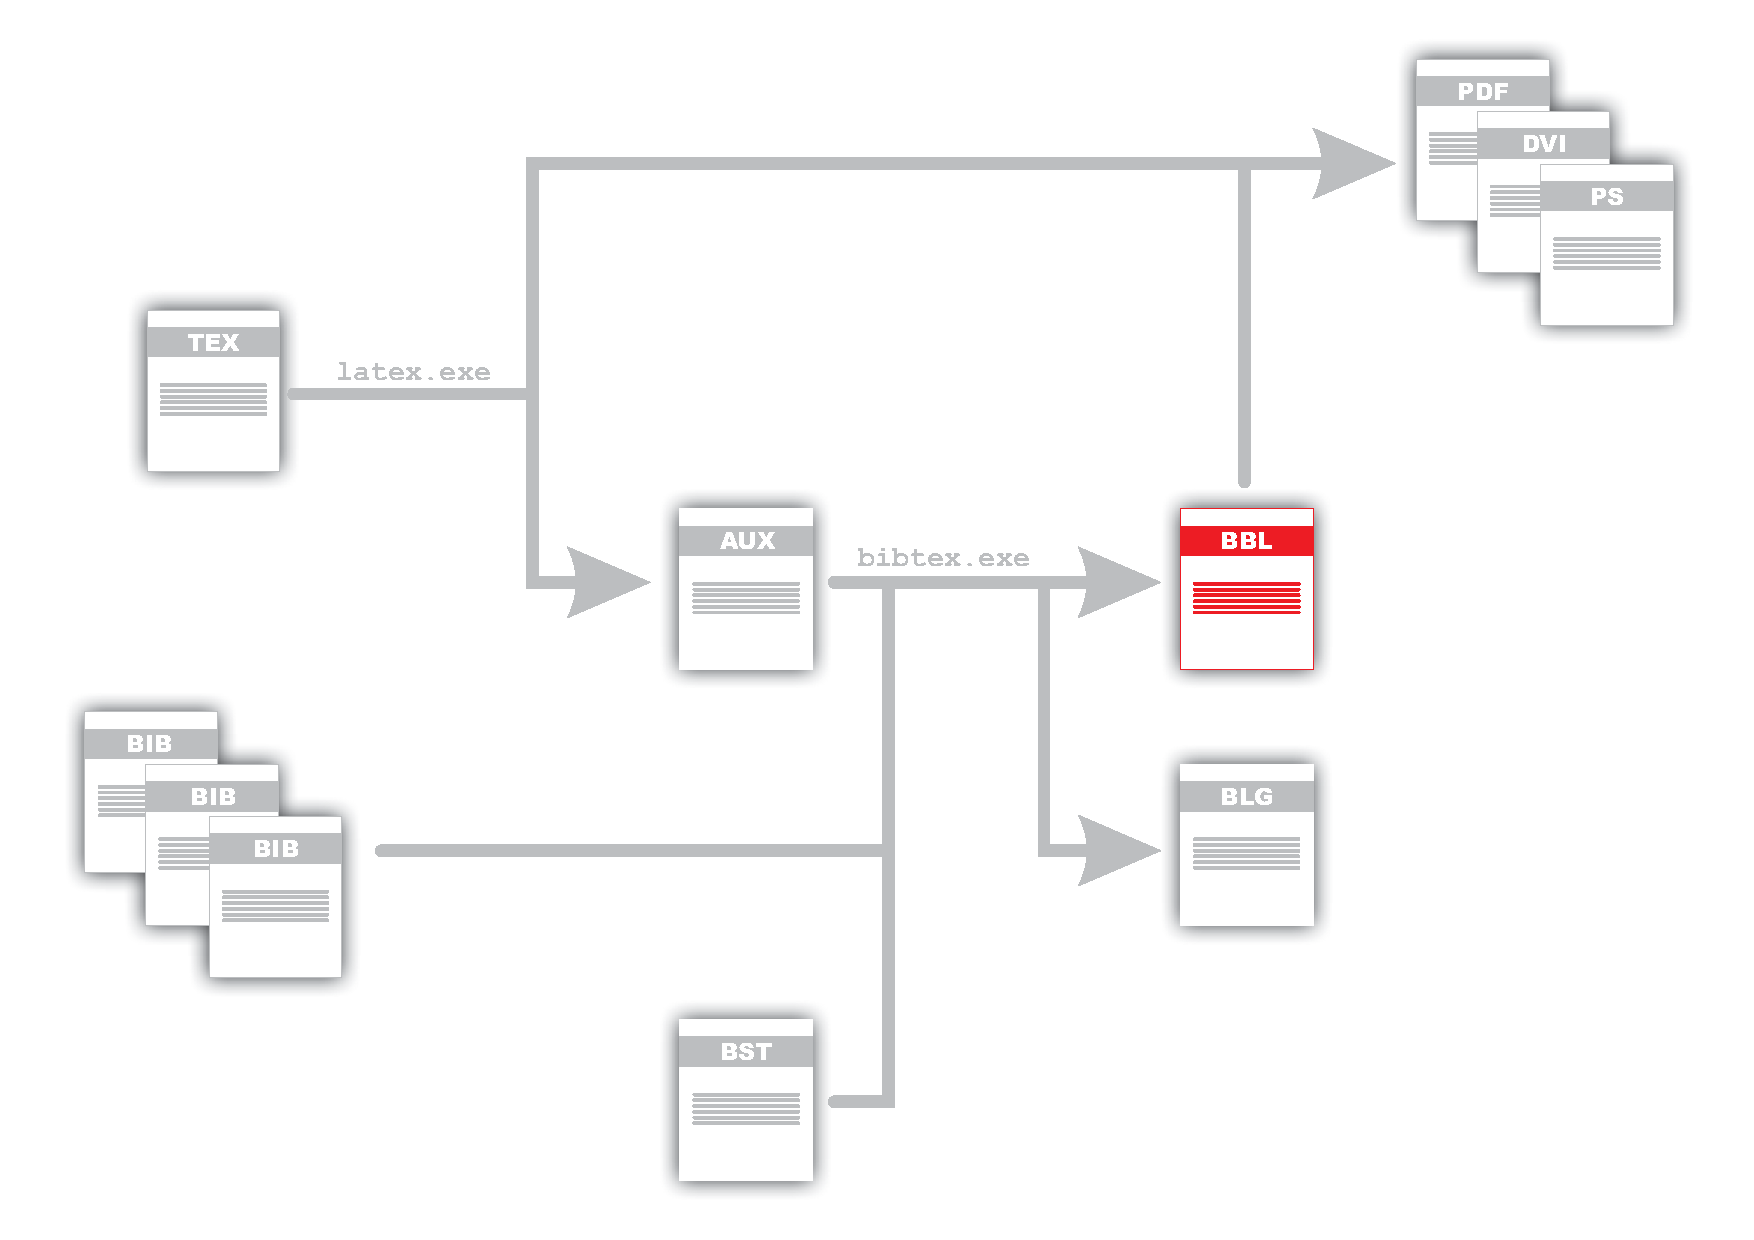
\includegraphics[height=0.55\textheight]{bibfiles_bbl}}}
\newsavebox{\blgbox}
\savebox{\blgbox}{\raisebox{-0.5\height}[0.5\height][0.25\height]{%
	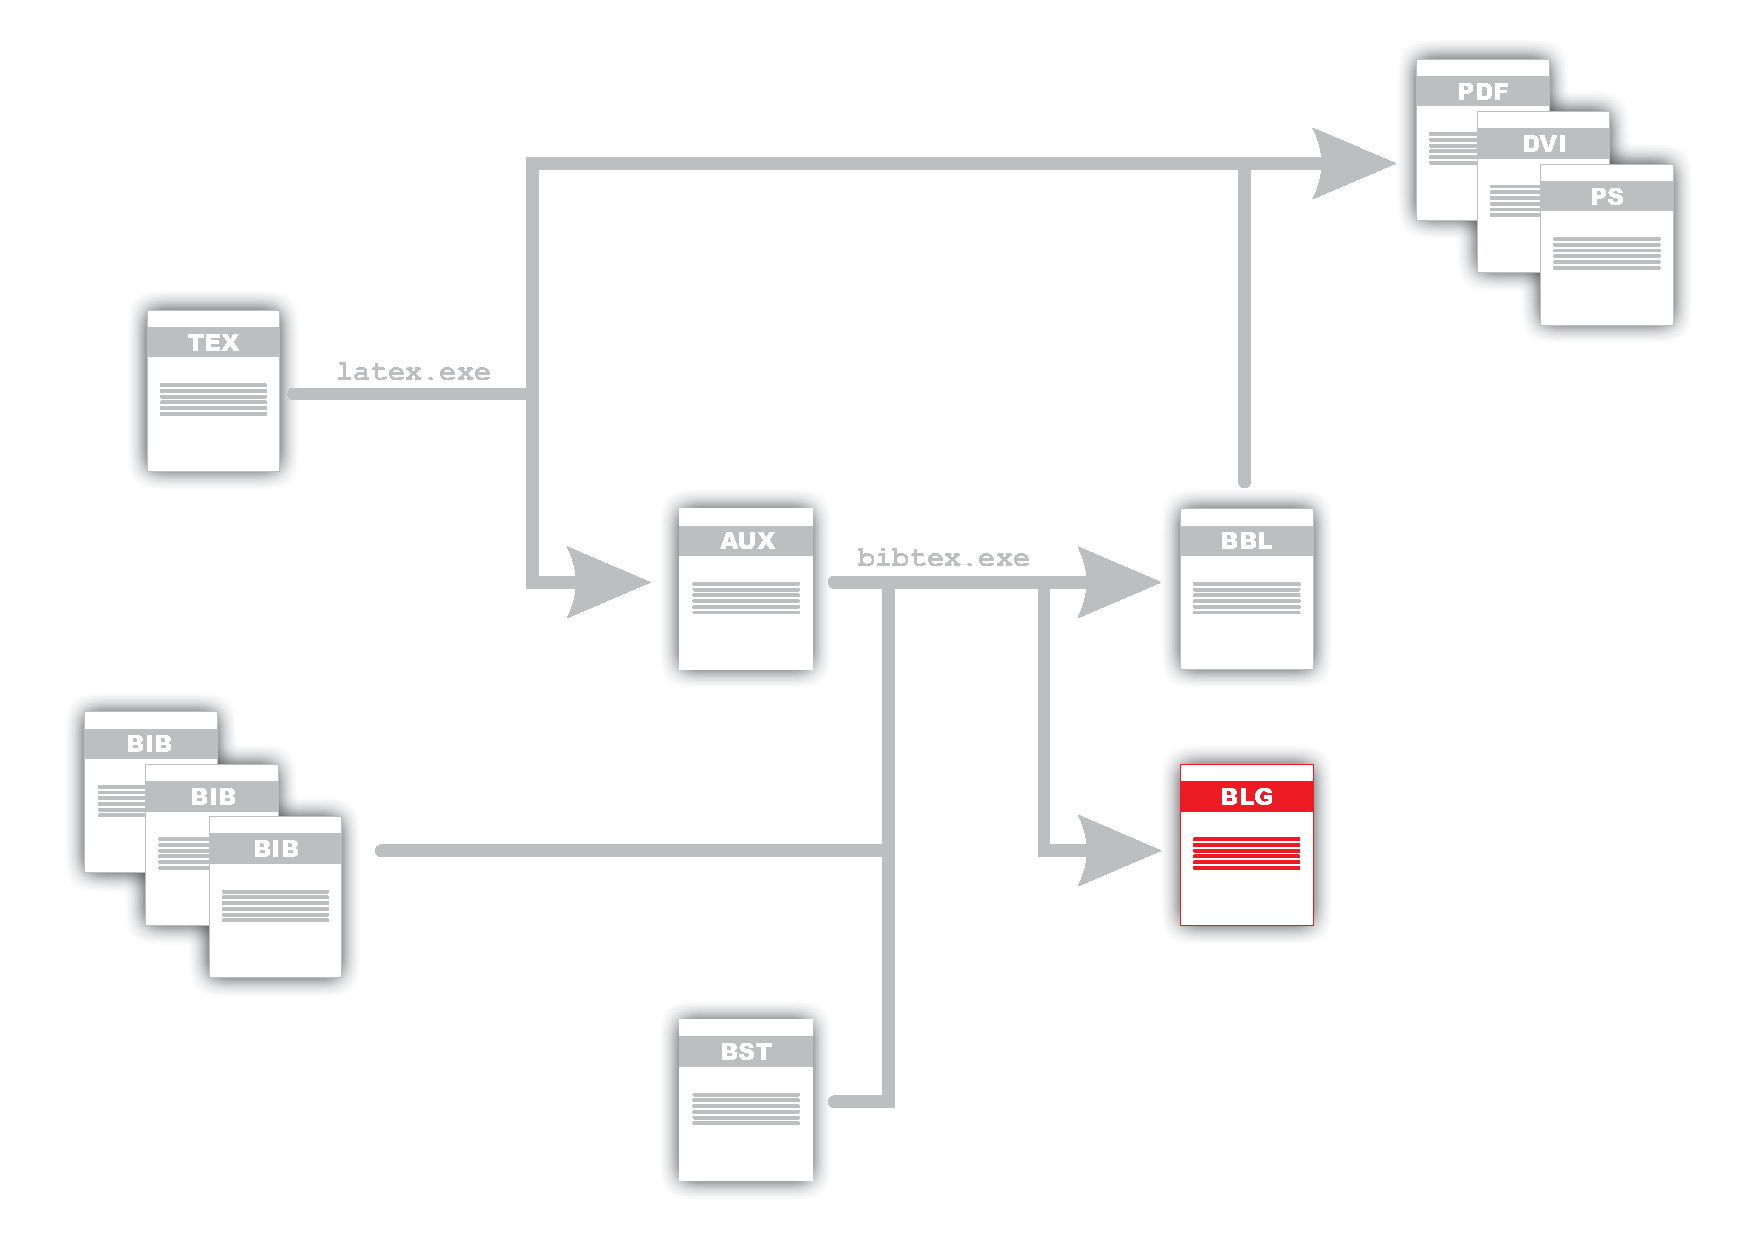
\includegraphics[height=0.55\textheight]{bibfiles_blg}}}
	
\subsection{Os arquivos envolvidos}
\begin{frame}
	\frametitle{\bibtex}
	\framesubtitle{Os arquivos}
	
	\begin{flushright}
		\onslide<1>{\usebox{\bibbox}}%
		\onslide<2>{\llap{\usebox{\bstbox}}}%
		\onslide<3>{\llap{\usebox{\bblbox}}}%
		\onslide<4->{\llap{\usebox{\blgbox}}}%
	\end{flushright}
	
	\onslide<1->{Os arquivos do \bibtex:}
	\begin{itemize}
		\item<1->[\texttt{bib}] \alert<1>{A base de dados bibliográficos}
		\item<2->[\texttt{bst}] \alert<2>{O leiaute (ou estilo) de exibição}
		\item<3->[\texttt{bbl}] \alert<3>{\ambiente{thebibliography} gerado pelo
			\bibtex\ (\textbf{dados $+$ leiaute})}
		\item<4->[\texttt{blg}] \alert<4>{Arquivo de log gerado pelo \bibtex}
	\end{itemize}
\end{frame}
}
%-------------------------------------------------------------------
\subsection{Usando o \bibtex}
\begin{frame}[fragile]
	\frametitle{\bibtex}
	\frametitle{Utilização}
	
	\onslide<1->{No lugar da lista \texttt{thebibliography}, \dots}
	
	\begin{enumerate}
		\item<1-> Informe onde estão seus dados bibliográficos:
		
			\begin{columns}
				\column{0.8\textwidth}
					\begin{block}<2->{}
						\cs{bibliography}%
							\verb|{|%
						\textit{arquivo \texttt{bib} 1, arquivo \texttt{bib} 2, \dots}%
							\verb|}|
					\end{block}
			\end{columns}
						
		\item<3-> e escolha o leiaute de exibição deles (apenas um):
			
			\begin{columns}
				\column{0.8\textwidth}
					\begin{block}<3->{}
						\cs{bibliographystyle}%
							\verb|{|%
						\textit{arquivo \texttt{bst}}%
							\verb|}|
					\end{block}
			\end{columns}
			
		\medskip
		
		\footnotesize\textbf{obs.:} \emph{não} informe a extensão dos arquivos.
	\end{enumerate}\vfill
	
	\begin{atividade}<4->{2}
		Estude o arquivo \texttt{Atividade02.tex} (\alert<4>{não o compile ainda}).
	\end{atividade}
	
\end{frame}
%-------------------------------------------------------------------
\newsavebox{\bibentry}
\savebox{\bibentry}{\parbox{0.3\textwidth}{%
	\textcolor{red}{\texttt{@}}\textit{tipo}%
	\textcolor{red}{\texttt{(}}\textit{rótulo}%
	\textcolor{red}{\texttt{,}}\\
	\rule{0.5cm}{0pt}\textit{campo }%
	\textcolor{red}{\texttt{=}}\textit{ valor}%
	\textcolor{red}{\texttt{,}}\\
	\rule{0.5cm}{0pt}\textit{campo }%
	\textcolor{red}{\texttt{=}}\textit{ valor}%
	\textcolor{red}{\texttt{,}}\\
	\rule{0.5cm}{0pt}\phantom{campo }\vdots\\
	\textcolor{red}{\texttt{)}}}}

\subsection{Entradas bibliográficas}
\begin{frame}[fragile]
	\frametitle{\bibtex}
	\framesubtitle{Entradas bibliográficas}

	A estrutura de uma entrada bibliográfica (pares chave-valor):
	
	\begin{columns}
		\centering
		\column{0.3\textwidth}
		\begin{block}{\begin{center}Arquivo \texttt{.bib}\end{center}}
			\centering
			\usebox{\bibentry}
		\end{block}
	\end{columns}
	
	\begin{description}
		\item<2->[\textit{tipo}] \texttt{book}, \texttt{article}, \texttt{phdthesis},
		etc\\ \hyperlink{tiposXcampos}{\footnotesize\color{blue}(%
		link: tipos $\times$ campos)}
		
		\item<3->[\textit{rótulo}] o nome usado por \verb|\cite|
		\item<4->[\textit{campo}] \texttt{author}, \texttt{title}, \texttt{date}, etc
		\item<5->[\textit{valor}] os dados propriamente ditos
	\end{description}
	
\end{frame}
%-------------------------------------------------------------------
\begin{frame}[fragile]\footnotesize
	\frametitle{\bibtex}
	\framesubtitle{Exemplo de entradas bibliográficas e regras}

	\begin{minipage}{\textwidth}\ttfamily
		\begin{LaTeXcode}
			@BOOK(Kopka:1999,
			  author = {Helmut Kopka and Patrick W. Daly},
			  title = {A guide to {\LaTeX}},
			  publisher = {Addison-Wesley},
			  year = 1999,
			)
		\end{LaTeXcode}
	\end{minipage}
			
	\begin{itemize}
		\item<2-> O \bibtex\ \emph{não} distingue maiúsculas de minúsculas\\
			{\tiny(para garantir a forma, use chaves: eg., \verb|{\LaTeX}| acima)}
			
		\item<3-> O \bibtex\ ignora os campos que não conhece\\
			{\tiny(use-os para comentários)}
			
		\item<4-> Valores são abertos (e fechadas) com parênteses ou com aspas
			(\alert<4>{\textquotedbl})\\
			{\tiny(valores numéricos podem ou não estar entre chaves ou aspas)}
			
		\item<5-> Pares campo-valor separados por vírgula\\
			{\tiny(\textbf{dica:} coloque vírgula no último campo)}
				
		\item<6-> No campo \texttt{author}, separe o nome dos autores por
			``\texttt{and}''\\
			{\tiny(\textbf{eg.:} fulano \texttt{and} sicrano \texttt{and} beltrano)}
	\end{itemize}
\end{frame}
%-------------------------------------------------------------------
\begin{frame}
	\small
	
	\begin{block}<1->{Exercício}
		Estude os arquivos \texttt{Atividade02.tex} e \texttt{Referencias.bib}
		e compile o arquivo \texttt{tex} \emph{três} vezes (até que não haja
		mais avisos do \LaTeX).
	\end{block}\vfill
	
	\begin{block}<2->{Exercício}
		Quais são os leiautes disponíveis na sua máquina?
	\end{block}\vfill
	
	\begin{block}<3->{Exercício}
		Crie o arquivo \texttt{minhasRef.bib} e, dentro dele, crie uma
		entrada bibliográfica no formato \bibtex. Depois, insira esta base de
		dados no comando \cs{bibliography} do arquivo \texttt{Atividade02.tex},
		cite-a e compile.
	\end{block}\vfill
	
	\begin{block}<4->{Exercício}
		Pegue uma entrada bibliográfica de um artigo num jornal qualquer, no
		formato \bibtex, e insira-a no seu documento. Faça uma citação e compile.	
	\end{block}
	
\end{frame}
%-------------------------------------------------------------------	
\subsection{\bibtex\ passo a passo}
\begin{frame}[fragile]\footnotesize
	\frametitle{\bibtex\ passo a passo}

	\begin{atividade}{3}
		\begin{enumerate}
			\item<2-> Compile o arquivo com o \LaTeX: \verb|latex Atividade02|
			
				\begin{itemize}
					\item<3-> Analise os avisos do \LaTeX
					\item<4-> Analise o arquivo \texttt{Atividade02.aux}\\
					(as referências ainda são desconhecidas)
				\end{itemize}
			
			\item<5-> Execute o \bibtex: \verb|bibtex Atividade02|
				
				\begin{itemize}
					\item<6-> Analise as mensagens do \bibtex\ (\texttt{.blg})
					\item<7-> Abra o arquivo \texttt{Atividade02.bbl}
				\end{itemize}
				
			\item<8-> Reexecute \LaTeX: \verb|latex Atividade02|
			
				\begin{itemize}
					\item<9-> Reveja o arquivo \texttt{Atividade.aux}\\
						(as referências agora são conhecidas)
				\end{itemize}
						
			\item<10-> Execute o \LaTeX\ novamente
		\end{enumerate}
	\end{atividade}
\end{frame}
%-------------------------------------------------------------------
\subsection{JabRef}
\begin{frame}
	\frametitle{JabRef}
	\framesubtitle{Uma interface gráfica para o \bibtex}
	
	\begin{atividade}{}
		Baixe e instale o JabRef
		(\href{http://cepa.if.usp.br/ivan/LaTeX/JabRef/}{%
		\color{blue}clique aqui}).
	\end{atividade}\vfill

	\begin{atividade}<2->{}
		Use o JabRef para abrir os arquivos \texttt{Referencias.bib} e
		\texttt{minhareferencia.bib}
	\end{atividade}\vfill
	
	\begin{atividade}<3->{}
		Insira uma nova referência em qualquer um dos arquivos através do JabRef e
		cite-a no \texttt{Atividade02.tex}
	\end{atividade}

\end{frame}
%-------------------------------------------------------------------
\section{Ligações}
\subsection{Letras: ff, fi, etc}

\begin{frame}[fragile]
	\frametitle{Ligações (\foreign{ligatures})}
	\framesubtitle{Letras}
	
	\begin{block}{}
		\centering
		São seqüências de caracteres substituídos por outro(s).
	\end{block}\vfill
	
	\pause
	
	\begin{center}
		\begin{tabular}{lccccc}
			\toprule		
			& \verb|ff| & \verb|fi| & \verb|fl| & \verb|ffi| & \verb|ffl| \\
			\cmidrule{1-6}
			
			C. Modern & \huge\cmr ff & \huge\cmr fi & \huge\cmr fl & \huge\cmr ffi & 
				\huge\cmr ffl \\
				
			Utopia & \huge ff & \huge \alert<3>{fi} & \huge \alert<3>{fl} &
				\huge ffi & \huge ffl \\
				
			\cmidrule{1-6}
			& \cmr effect & \cmr ficar & \cmr flexível & \cmr efficient &
				\cmr offline \\
				
			\bottomrule
		\end{tabular}
	\end{center}\vfill
	
	\onslide<4->{Para evitar, coloque \texttt{\{\}} entre as letras:}
	\begin{itemize}
		\item<4-> \verb|f{}lexível| produz ``f{}lexível'' ao invés de
			``\alert<4>{fl}exível''
		\item<5-> \verb|f{}icar| produz ``f{}icar'' ao invés de 
			``\alert<5>{fi}car''
	\end{itemize}
	
\end{frame}
%-------------------------------------------------------------------
\subsection{Hífen, travessão etc}
\begin{frame}[fragile]
	\frametitle{Ligações (\foreign{ligatures})}
	\framesubtitle{Hífen, travessão, etc.}

	\begin{center}
		\begin{tabular}{ccl}
			\toprule
			Seqüência & Produz & Função \\
			\midrule
			\verb|-|   & -   & Hífen                         \\
			\verb|--|  & --  & Intervalo (\foreign{en-dash}) \\
			\verb|---| & --- & Travessão (\foreign{em-dash}) \\
			\verb|$-$| & $-$ & Subtração                     \\
			\bottomrule
		\end{tabular}
	\end{center}\vfill
		
	\begin{itemize}\small
		\item<2-> Matéria-prima, guarda-chuva; diga-me, etc.
		\item<3-> pp.~6--8; 15--\unit{23}{\celsius}
		\item<4->
			\begin{minipage}[c]{0.3\textwidth}
				\footnotesize\itshape
					A moça hesitava:\\
					--- Experimente!
					
					\tiny\upshape\hfill \textbf{Senhora}, de José de Alencar			
			\end{minipage}\hfill
			\begin{minipage}[c]{0.55\textwidth}
				\footnotesize\itshape
				Com o fim de mostrar que valia mais que	os outros, --- e acaso para
				reconciliar-se com o céu --- compôs a partitura, (\dots)
			
				\tiny\upshape\hfill \textbf{Dom Casmurro}, de Machado de Assis				
			\end{minipage}
		\item<5-> $3 - 2 = 1$
	\end{itemize}
\end{frame}
%-------------------------------------------------------------------
\newcommand{\aspas}{\raisebox{-1ex}{
\includegraphics[height=3ex]{key_aspas}}}
\newcommand{\crase}{\raisebox{-1ex}{
\includegraphics[height=3ex]{key_crase}}}
\newcommand{\agudo}{\raisebox{-1ex}{
\includegraphics[height=3ex]{key_agudo}}}
\newcommand{\apostrofo}{\raisebox{-1ex}%
	{
\includegraphics[height=3ex]{key_apostrofo}}}

\subsection{Aspas e apóstrofo}
\begin{frame}[fragile]
	\frametitle{Ligações (\foreign{ligatures})}
	\framesubtitle{Aspas e apóstrofo}
	
	\centering
	
	\begin{columns}
		
		\column{0.40\textwidth}
			\centering
			\begin{tabular}{ccc}
				\toprule
				Seqüência & Produz & Exemplo \\
				\midrule		
				\crase & ` & \\
				\aspas & ' & \raisebox{1.5ex}[0pt]{`texto'}\\
				\cmidrule{1-3}
				\crase\crase & `` & \\	
				\aspas\aspas & '' & \raisebox{1.5ex}[0pt]{``texto''}\\		
				\bottomrule			
			\end{tabular}

		\column{0.15\textwidth}
			\centering
			\onslide<1->{
\includegraphics[width=\textwidth]{keystrokes}}
					
	\end{columns}\vfill
	
	\begin{block}<2->{}
		\centering\Large
		\begin{tabular}{c!{$\quad\to\quad$}c}
			\crase\texttt{texto}\aspas             & `texto' \\
			\crase\crase\texttt{texto}\aspas\aspas &``texto''
		\end{tabular}
	\end{block}
	
			
\end{frame}
%-------------------------------------------------------------------
\begin{frame}[fragile]
	\frametitle{Ligações (\foreign{ligatures})}
	\framesubtitle{Aspas e apóstrofo}
	
	\begin{tabular}{l!{\quad produz\quad}l}
		\multicolumn{2}{l}{\onslide<1->\textbf{Erros comuns:}} \\
		\onslide<1->\aspas\verb|texto|\aspas & 'texto' \\
		\onslide<2->\crase\verb|texto|\crase & `texto` \\
		\onslide<3->\agudo\verb|texto|\agudo & ´texto´ \\
		\onslide<4->\apostrofo\verb|texto|\apostrofo & "texto"	\\
		\multicolumn{2}{c}{}\\			
		\multicolumn{2}{l}{\onslide<5->\textbf{Dicas:}}\\
		\onslide<5->\verb|```a' e `b'''|       & \textcolor{red}{``}`a' e
			`b\textcolor{red}{''}' \\
		\onslide<6->\verb|``{}`a' e `b'{}''| & ``{}`a' e `b'{}'' \\		
		\onslide<7->\verb|``\,`a' e `b'\,''| & ``\,`a' e `b'\,'' \\		
		\onslide<8->\verb|texto.''|          & texto.'' \\
		\onslide<9->\verb|texto''.|          & texto''. \\
		\onslide<10->\verb|texto\rlap{.}''|   & texto\rlap{.}''
	\end{tabular}
			
\end{frame}
%-------------------------------------------------------------------
\section{Final de frase}
\subsection{A regra}
\begin{frame}[fragile]
	\frametitle{Final de frase}
	
	\begin{block}{Regra tipográfica}
		Alocar mais espaço entre \emph{frases} (ie., no final delas)
	\end{block}\vfill
	
	\begin{block}<2->{Regra do \LaTeX\ para identificar final de frases}
		Os \emph{caracteres} ponto-final (.), interrogação (?),	exclamação (!) e
		dois-pontos (:) têm a \emph{função} de marcar o final de uma frase, a 
		menos que sejam precedidos por uma letra maiúscula. Neste caso o \LaTeX\
		interpreta a \emph{palavra} anterior como uma abreviação e a frase
		continua.
	\end{block}\vfill
	
	\begin{columns}
	
		\scriptsize
		\centering
	
		\column{0.45\textwidth}
			\centering
		
			\setbox1=\hbox to 1.0\textwidth{Esta é uma oração. E outra.}
			\setbox2=\hbox to 0.9\textwidth{Esta é uma oração. E outra.}
			\setbox3=\hbox to 0.8\textwidth{Esta é uma oração. E outra.}
			\setbox4=\hbox to 0.7\textwidth{Esta é uma oração. E outra.}	
			
			\begin{uncoverenv}<3->
				\box1		
				\box2		
				\box3		
				\box4
			\end{uncoverenv}
		
		\column{0.05\textwidth}
			\centering
			\onslide<4->{\rule{0.1pt}{2cm}}
			
		\column{0.45\textwidth}
			\centering
			\setbox1=\hbox to 1.0\textwidth{Esta é uma oração, E outra.}
			\setbox2=\hbox to 0.9\textwidth{Esta é uma oração, E outra.}
			\setbox3=\hbox to 0.8\textwidth{Esta é uma oração, E outra.}
			\setbox4=\hbox to 0.7\textwidth{Esta é uma oração, E outra.}
		
			\begin{uncoverenv}<4->
				\box1		
				\box2		
				\box3		
				\box4
			\end{uncoverenv}
			
	\end{columns}			
\end{frame}
%-------------------------------------------------------------------
\subsection{1\textordfeminine\ exceção}
\begin{frame}[fragile]
	\frametitle{Final de frase}
	
	\begin{center}
		\begin{tikzpicture}
		\node [rectangle,rounded corners=1mm,minimum size=7mm,very thin,
			draw=red, top color=red!20,bottom color=white!20]
			{1\textordfeminine\ exceção: ponto-final no meio da frase.};
		\end{tikzpicture}
	\end{center}\vfill
		
	\begin{columns}
		\scriptsize
		
		\column{0.45\textwidth}
			\centering
			\setbox1=\hbox to 1.0\textwidth{Fulano et al. fizeram isso.}
			\setbox2=\hbox to 0.9\textwidth{Fulano et al. fizeram isso.}
			\setbox3=\hbox to 0.8\textwidth{Fulano et al. fizeram isso.}
			\setbox4=\hbox to 0.7\textwidth{Fulano et al. fizeram isso.}	
			
			\begin{uncoverenv}<1->
				\box1		
				\box2		
				\box3		
				\box4
			\end{uncoverenv}
			
		\column{0.05\textwidth}
			\centering
			\onslide<3->{\rule{0.1pt}{2cm}}
			
		\column{0.45\textwidth}
			\centering
			\setbox1=\hbox to 1.0\textwidth{Fulano et al.\ fizeram isso.}
			\setbox2=\hbox to 0.9\textwidth{Fulano et al.\ fizeram isso.}
			\setbox3=\hbox to 0.8\textwidth{Fulano et al.\ fizeram isso.}
			\setbox4=\hbox to 0.7\textwidth{Fulano et al.\ fizeram isso.}
				
			\begin{uncoverenv}<3->
				\box1		
				\box2		
				\box3		
				\box4
			\end{uncoverenv}	
	\end{columns}\vfill
	
	\begin{block}<2->{\begin{center}Solução\end{center}}
		\centering
		Revogue a \emph{função} ``ponto-final'' do \emph{caráter} ponto-final:\\
		\ttfamily Fulano de tal et al.{\color{red}\verb*|\ |}fizeram isso.
	\end{block}
	
	\vfill
	
	\scriptsize
	\textcolor{gray}{obs.\,: ``et al'' vem do latim e significa ``e 
	colaboradores\rlap{.}''}
	
\end{frame}
%-------------------------------------------------------------------
\subsection{2\textordfeminine\ exceção}
\begin{frame}[fragile]
	\frametitle{Final de frase}
		
	\begin{center}
		\begin{tikzpicture}
		\node [rectangle,rounded corners=1mm,minimum size=7mm,very thin,
			draw=red, top color=red!20,bottom color=white!20]
			{2\textordfeminine\ exceção: a frase termina com maiúscula.};
		\end{tikzpicture}
	\end{center}\vfill
	
	\begin{columns}
		\column{0.45\textwidth}
			\scriptsize
			\setbox1=\hbox to 1.0\textwidth{João Paulo II. O Grande?}
			\setbox2=\hbox to 0.9\textwidth{João Paulo II. O Grande?}
			\setbox3=\hbox to 0.8\textwidth{João Paulo II. O Grande?}
			\setbox4=\hbox to 0.7\textwidth{João Paulo II. O Grande?}	
		
			\begin{uncoverenv}<1->
				\box1		
				\box2		
				\box3		
				\box4
			\end{uncoverenv}
			
		\column{0.05\textwidth}
			\onslide<3->{\rule{0.1pt}{2cm}}
				
		\column{0.45\textwidth}
			\scriptsize
			\setbox1=\hbox to 1.0\textwidth{João Paulo II\@. O Grande?}
			\setbox2=\hbox to 0.9\textwidth{João Paulo II\@. O Grande?}
			\setbox3=\hbox to 0.8\textwidth{João Paulo II\@. O Grande?}
			\setbox4=\hbox to 0.7\textwidth{João Paulo II\@. O Grande?}
					
			\begin{uncoverenv}<3->
				\box1		
				\box2		
				\box3		
				\box4
			\end{uncoverenv}	
	\end{columns}\vfill
	
	\begin{block}<2->{\begin{center}Solução\end{center}}
		\centering
		Reatribua a \emph{função} ``ponto-final'' ao \emph{caráter} ponto-final:\\
		\ttfamily João Paulo II{\color{red}\verb|\@|}. O Grande?
	\end{block}
		
\end{frame}
%-------------------------------------------------------------------
\subsection{Caso particular}
\begin{frame}[fragile]
	\frametitle{Final de frase}
				
	\begin{center}
		\begin{tikzpicture}
		\node [rectangle,rounded corners=1mm,minimum size=7mm,very thin,
			draw=red, top color=red!20,bottom color=white!20]
			{Caso particular: o espaço se propaga através das aspas};
		\end{tikzpicture}
	\end{center}\vfill
				
	\begin{columns}
		\scriptsize
		\column{0.45\textwidth}
			\setbox1=\hbox to 1.0\textwidth{``um, dois, etc.'' e continua.}
			\setbox2=\hbox to 0.9\textwidth{``um, dois, etc.'' e continua.}
			\setbox3=\hbox to 0.8\textwidth{``um, dois, etc.'' e continua.}
			\setbox4=\hbox to 0.7\textwidth{``um, dois, etc.'' e continua.}
		
			\begin{uncoverenv}<1->
				\box1		
				\box2		
				\box3		
				\box4
			\end{uncoverenv}
		
		\column{0.05\textwidth}
			\onslide<3->{\rule{0.1pt}{1.5cm}}
		
		\column{0.45\textwidth}
			\setbox1=\hbox to \textwidth{``um, dois, etc.''\ e continua.}
			\setbox2=\hbox to 0.9\textwidth{``um, dois, etc.''\ e continua.}
			\setbox3=\hbox to 0.8\textwidth{``um, dois, etc.''\ e continua.}
			\setbox4=\hbox to 0.7\textwidth{``um, dois, etc.''\ e continua.}
										
			\begin{uncoverenv}<3->
				\box1		
				\box2		
				\box3		
				\box4
			\end{uncoverenv}	
	\end{columns}\vfill
	
	\begin{block}<2->{\begin{center}Solução\end{center}}
		\centering
		Use \verb*|\ | \textcolor{red}{após} as aspas (ou \verb|\rlap|):\\
		\ttfamily \verb|``|um, dois, etc.{\color{red}\verb*|''\ |}e continua.\\
		\verb|``|um, dois, etc{\color{red}\verb*|\rlap{.}''|} e continua.
	\end{block}
	
\end{frame}
%-------------------------------------------------------------------
\begin{frame}[fragile]
	\frametitle{Final de frase}
		
	\begin{center}
		\begin{tikzpicture}
		\node [rectangle,rounded corners=1mm,minimum size=7mm,very thin,
			draw=red, top color=red!20,bottom color=white!20]
			{Caso particular: o espaço se propaga através do parêntese};
		\end{tikzpicture}
	\end{center}\vfill
			
	\begin{columns}
		\scriptsize
		\column{0.45\textwidth}
			\setbox1=\hbox to 1.0\textwidth{Beans (lima, etc.) have vitamin B.}
			\setbox2=\hbox to 0.9\textwidth{Beans (lima, etc.) have vitamin B.}
			\setbox3=\hbox to 0.8\textwidth{Beans (lima, etc.) have vitamin B.}
			
			\begin{uncoverenv}<1->
				\box1		
				\box2		
				\box3		
			\end{uncoverenv}
			
		\column{0.05\textwidth}
			\onslide<3->{\rule{0.1pt}{1cm}}
			
		\column{0.45\textwidth}
			\setbox1=\hbox to 1.0\textwidth{Beans (lima, etc.)\ have vitamin B.}
			\setbox2=\hbox to 0.9\textwidth{Beans (lima, etc.)\ have vitamin B.}
			\setbox3=\hbox to 0.8\textwidth{Beans (lima, etc.)\ have vitamin B.}
								
			\begin{uncoverenv}<3->
				\box1		
				\box2		
				\box3		
			\end{uncoverenv}
	\end{columns}\vfill
	
	\begin{block}<2->{\begin{center}Solução\end{center}}
		\centering
		Use \verb*|\ | \textcolor{red}{após} as chaves:\\
		\ttfamily Beans (lima, etc.){\color{red}\verb*|\ |}have vitamin B.
	\end{block}
\end{frame}
%-------------------------------------------------------------------
\section{Espaços indivisíveis}
\begin{frame}[fragile]
	\frametitle{Espaços indivisíveis: o til (\~{})}

	\begin{block}{}
		\centering
		Use \~{} (til) para representar um espaço indivisível
	\end{block}
	
	Regras~\cite{TeXbook}:
	\begin{itemize}
		\item<1-> Partes do documento:\\
		\color{blue}\verb|capítulo~3|\color{black},\qquad
		\color{blue}\verb|fig.~\ref{rotulo}|\color{black}, etc
		
		\item<2-> Entre nomes:\\
		\color{blue}\verb|Donald~E. Knuth|\color{black},\qquad
		\color{blue}\verb|D.~Pedro~II|\color{black}, etc
		
		\item<3-> Entre substantivos e o símbolo matemático associado:\\
		\color{blue}\verb|velocidade~$v$|\color{black},\qquad
		\color{blue}\verb|função~$f(x)$|\color{black}, etc
		
		\item<4-> Entre símbolos numa série:\\
		\color{blue}\verb|1,~2 ou~3|\color{black},\qquad
		\color{blue}\verb|$a$,~$b$ e~$c$|\color{black}, etc
		
		\item<5-> Entre preposição e o símbolo matemático associado:\\
		\color{blue}\verb|de 0 a~1|\color{black},\qquad
		\color{blue}\verb|$f$ é função de~$x$|\color{black}, etc		
	\end{itemize}
\end{frame}
%-------------------------------------------------------------------
\ifhandout\else
	\logo{
\includegraphics[width=0.25\textwidth]{LogotipoCursoLaTeX_v3_pequeno}}
	\setbeamertemplate{background canvas}{}
	\againframe{titulo} % Reapresenta a página inicial.
\fi
%-------------------------------------------------------------------
\appendix
\begin{frame}[label=tiposXcampos]
	\frametitle{Tipos de entradas bibliográficas}
	\framesubtitle{e seus campos}
	
	\footnotesize
	
	\begin{block}{\texttt{@article}}
	\bfseries author, title, journal, year, pages, \mdseries volume, number,
	language, note
	\end{block}\vfill
	
	\begin{block}{\texttt{@book}}
	\bfseries author (ou editor), title, publisher, year, \mdseries edition,
	volume, series, number, address, month, language, note
	\end{block}\vfill
	
	\begin{block}{\texttt{@inproceedings} (\foreign{proceedings} de
	conferências)}
	\bfseries author, title, booktitle, year, \mdseries address, editor, volume, 
	series, number, organization, publisher, month, note, pages, language
	\end{block}\vfill
	
	\begin{block}{\texttt{@masterthesis} e \texttt{@phdthesis}}
	\bfseries author, title, school, year, \mdseries type, address, monty, note,
	pages (para \texttt{phdthesis} apenas)
	\end{block}\vfill
	
	\tiny
	\textbf{obs.:} os campos obrigatórios estão em negrito.
	
\end{frame}
%-------------------------------------------------------------------
\begin{frame}
	\frametitle{Referências}

	\begin{thebibliography}{-}
	
	  \bibitem{Kopka:1999}          % Rótulo
	    H. Kopka e P. W. Daly,      % Autor(es)
	    \textsl{A guide to \LaTeX}, % Título
	    Addison-Wesley              % Editora
	    (1999).                     % Ano
	    
	  \bibitem{Gratzer:1996}        % Rótulo
	   	G. Grätzer,                 % Autor(es)
	   	\textbf{Math into \LaTeX},  % Título
	   	\textit{Birkhäuser}         % Editora
	   	(1996).                     % Ano
	   				
	  \bibitem{TeXbook}                        % Rótulo
   		D.~E. Knuth,                           % Autor(es)
   		\textbf{The {\TeX}book},               % Título
   		\textit{American Mathematical Society} % Editora
   		(1984).                                % Ano
	\end{thebibliography}
\end{frame}
\end{document}